\chapter{Analisi}
\label{ch:analisi} %Label of the chapter lit rev. The key ``ch:lit_rev'' can be used with command \ref{ch:lit_rev} to refer this Chapter.
\section{Obiettivi}
I principali requisiti funzionali e obiettivi del sistema sono:

\begin{itemize}
    \item \textbf{Costruzione di un'architettura a micro-servizi}.

    \item \textbf{Autenticazione e registrazione utenti: } possibilità di accedere ad un'area privata per poter visualizzare informazioni personali, oltre alla possibilità di poter giocare senza un proprio account in modalità 'ospite'.
    \item \textbf{Creazione e gestione partita: } gli utenti possono creare o partecipare ad una partita che inizierà soltanto quando 4 giocatori saranno presenti e disposti in due squadre da 2.

    \item \textbf{Chat di gioco: } possibilità di scambiare messaggi.

    \item \textbf{Nuova modalità di gioco} in cui se si commette un errore di gioco la partita viene conclusa conferendo alla squadra avversaria il massimo dei punti.

    \item \textbf{Persistenza dei dati: } salvataggio su database degli utenti e delle statistiche delle partite (mani giocate, briscola, etc...).
\end{itemize}
\section{Politiche di autovalutazione} 
Di seguito vengono riportati i casi che dovranno essere gestiti dal sistema:
\begin{itemize}
    \item l'elenco delle partite iniziate/finite deve rimanere aggiornato
    \item se un giocatore si disconnette la partita termina per tutti 
    \item connessione lenta o malfunzionamenti da parte di un giocatore
    \item un giocatore clicca sul tasto "esci"
    \item nel caso di un crash di un servizio si deve garantire che il servizio venga riavviato in automatico evitando che il sistema si blocchi
\end{itemize}
% Si devono seguire le regole per completare una sessione di gioco.
% • Se un giocatore che non `e l’ultimo rimasto si disconnette si disconnette la
% partita deve continuare. Nel caso in cui la partita fosse ancora in e il giocatre disconneso si volesse riconnettere il server far`a in modo di mostrare
% al giocatre le carte che aveva al momento della disconnessione
% • Se l’ultimo giocatore si disconnette allora la partita deve terminare.
% • L’elenco delle partite aperte/chiuse deve rimanere aggiornato. Inoltre,
% devono essere costantemente sincronizzati i client dei giocatori all’interno
% della stessa partita, in modo da garantire la coerenza del gioco.
% • L’obiettivo principale del software sviluppato `e garantire una solida capacit`a di adattamento alle dimensioni, una fluidit`a accettabile nell’esperienza
% di gioco e una sufficiente resilienza agli errori. In modo specifico, il servizio web necessita di gestire in modo efficace un grande numero di utenti
% simultaneamente, mentre l’esecuzione del gioco deve risultare scorrevole
% sul dispositivo dell’utente, evitando inconvenienti legati alle prestazioni sia
% grafiche che funzionali. Inoltre, `e essenziale che il sistema non si blocchi
% in caso di eventuali problemi.

\section{Requisiti e casi d'uso}
\subsection{Requisiti}
\begin{enumerate}
    \item Account
        \begin{enumerate}
            \item Login
            \item Registrazione
            \item Recupero password
            \item Visualizzazione profilo
            \item Modifica password
            \item Possibilità di scegliere se giocare come ospite o effettuare il login
        \end{enumerate}
    \item Realizzazione partita
        \begin{enumerate}
            \item Creazione partita
            \item Partecipazione partita
            \item gioca carta
            \item Inizio partita
            \item Fine mano
            \item Fine partita
        \end{enumerate}
    \item Chat di gioco
        \begin{enumerate}
            \item chat globale
            \item chat partita
        \end{enumerate}
    \item Possibilità di scegliere un compagno di squadra
    \item Scelta del seme, parole consentite
    \item Modalità di gioco 11 a 0
    \item Gestione punteggio
        \begin{enumerate}
            \item Calcolo totale e parziale (Gestione per ogni mano) del punteggio
            \item Maraffa/Cricca (+3 punti)
        \end{enumerate}
    \item Servizio gestione utenti
    \item Salvataggio statistiche
    \item Realizzazione GUI
        \begin{enumerate}
            \item Refactor della GUI esistente
            \item Rinnovamento GUI
        \end{enumerate}
\end{enumerate}
\subsection{Casi d'uso}
Si riporta di seguito lo schema dei casi d'uso che modella l'interazione dell'utente con l'applicazione.
\begin{figure}[h!]
    \centering 
    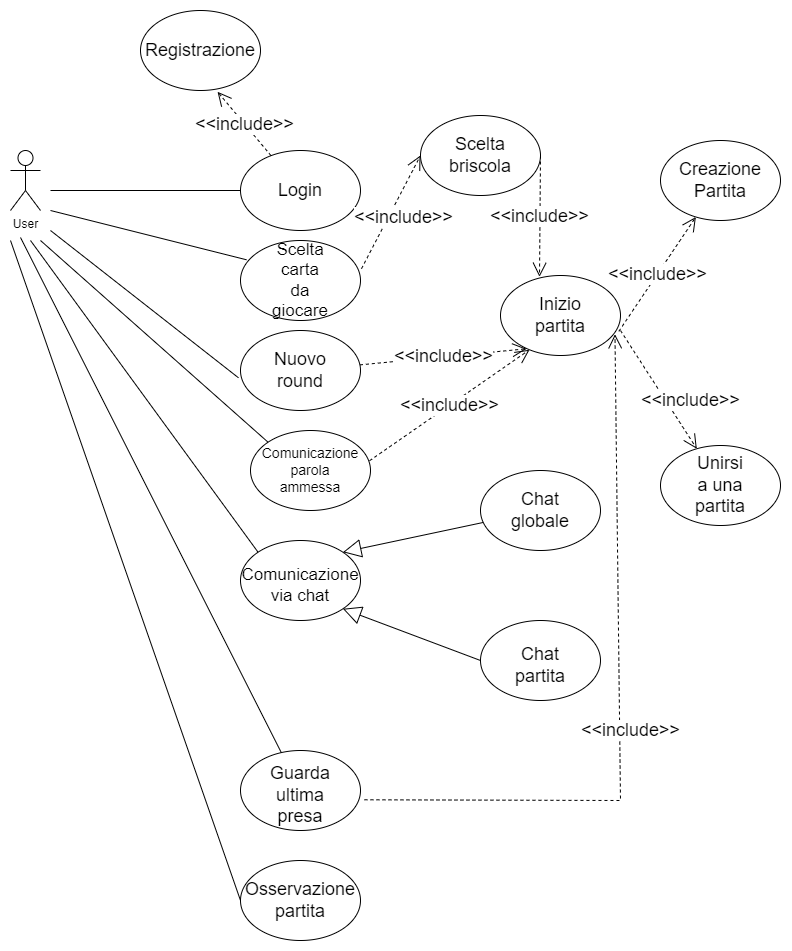
\includegraphics[scale=0.45]{report/img/Casi_duso.png}
    \caption{Casi d'uso}
    \label{use_case}
\end{figure}

% Take a note of the commands \textbackslash cite\{\} and \textbackslash citep\{\}. The command \textbackslash cite\{\} will write like ``Author et al. (2019)'' style for Harvard, APA and Chicago style. The command \textbackslash citep\{\} will write like ``(Author et al., 2019).'' Depending on how you construct a sentence, you need to use them smartly. Check the examples of \textbf{in-text citation} of sources listed here [This template recommends the \textbf{Harvard style} of referencing.]:
% \begin{itemize}
%     \item \cite{lamport1994latex} has written a comprehensive guide on writing in \LaTeX ~[Example of \textbackslash cite\{\} ].
%     \item If \LaTeX~is used efficiently and effectively, it helps in writing a very high-quality project report~\citep{lamport1994latex} ~[Example of \textbackslash citep\{\} ].   
%     \item A detailed APA, Harvard, and Chicago referencing style guide are available in~\citep{uor_refernce_style}.
% \end{itemize}




%\noindent
%\textbf{\color{red}MUST}: do read the university guidelines on the definition of plagiarism as well as the guidelines on how to avoid plagiarism~\citep{uor_plagiarism}.





